\chapter{The Alarm Screen}
\section{Overview}
The Alarm Screen is the screen the Operator uses to diagnose the Saw when it is in a Faulted State. It will provide information to the Operator about the nature of the Fault, and allow for acknowledgement of the faulted state by the Operator.
\begin{figure}
	\centering
	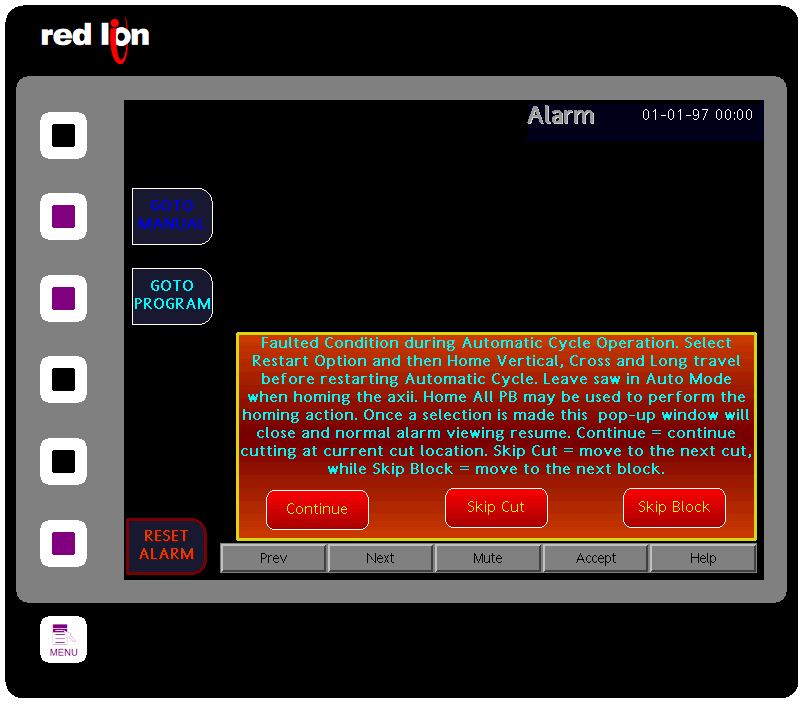
\includegraphics[width=0.75
	\linewidth]{screen-captures/alarms/alarms}
	\caption{Alarm Screen}
	\label{fig:alarm-screen}
\end{figure}
\pagebreak
\section{Alarm Screen Details}
The Alarm Screen details are divided into the following general categories.
\begin{list}{$\diamond$}{}
	\item \textbf{Screen Navigation}
	\item \textbf{Recovery Option Popup Window}
	\item \textbf{Alarm Acknowledge/Reset}
\end{list}
\subsection{Screen Navigation}Is performed by using the programmable Function Keys (FKeys) located down the left hand side of the OI Terminal (refer to Figure 2.2). The Operator may navigate to the \textbf{\textit{Manual Screen}} and the \textbf{\textit{Program Screen}}. and of course the \textbf{\textit{Main Screen}} using the \textit{Menu} FKey.
\begin{list}{$\diamond$}{}
	\item \textbf{GOTO MANUAL} Navigate to Manual Screen.
	\item \textbf{GOTO PROGRAM} Navigate to Cut Program Screen.
\end{list}
\begin{figure}
	\centering
	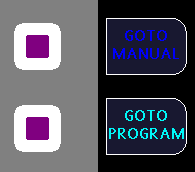
\includegraphics[width=.3\linewidth]{screen-captures/alarms/alarms-nav}
	\caption{Alarm Screen Navigation}
	\label{fig:alarm-nav}
\end{figure}
\paragraph*{\textbf{\LARGE \textcolor{blue}{i}}}
The Menu Key located on the terminal at the lower left below the FKey's, will return the Operator to the Main Screen, from all other screens.\\
\begin{minipage}{4cm}
	\begin{picture}(20,70)
	
\includegraphics[width=.5\linewidth]{screen-captures/menu}
	\end{picture}
\end{minipage}\begin{minipage}[]{11cm}
\paragraph{\textbf{\LARGE \textcolor{blue}{i}}} The Menu Key is pictured as it looks on the Terminal.
\end{minipage}
\pagebreak
\subsection{Alarm Recovery Popup Window} \paragraph*{This}window pops up if running in Automatic and an alarm condition occurs. It offers three choices to the Operator for recovery ... 
\begin{list}{$\diamond$}{}
	\item \textbf{Continue}
	\item \textbf{Skip Cut}
	\item \textbf{Skip Block}
\end{list}
The \textit{Alarm Recovery Popup Window} shown in Figure 2.3 will offer the Operator options on how to proceed from the alarmed condition back into running in automatic. If \textit{Continue} is chosen, the Operator would then reset the alarm and restart the automatic cycle and the saw will continue from the current location. This option relies on the Operator assessment of the safety to the equipment if starting from that particular state. By choosing to \textit{Skip Cut} the Operator is deciding to move onto the next cut location for the existing block being worked on by the program. This option will skip to the next cut location of the slab size being cut at the time of the faulted condition occurring. \textit{Skip Block} by extension is used to skip the current block and begin the cycle at the next block first cut location. This offers options to the Operator on how they wish to recover based on the condition of the bed of material and the saw itself.
\begin{figure}
	\centering
	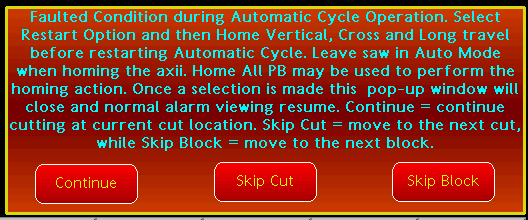
\includegraphics[width=.5\linewidth]{screen-captures/alarms/alarms-recovery}
	\caption{Alarm Recovery Popup Window}
	\label{fig:alarm-recovery}
\end{figure}
\subsection{Alarm Messages and Acknowledge/Reset} \paragraph*{The}\textbf{\textit{Alarm Reset}} pushbutton or the \textbf{\textit{Alarm Acknowledge Button}} are how the Operator acknowledges a Fault to clear it. The Operator \textbf{must} acknowledge \textbf{all} Faults in order to clear them. Faults must be cleared before the Operator can change the Saw into \textit{Auto Mode}. A number of faults clear whenever the faulted condition(s) are no longer present, these will remain until Acknowledged/Reset, but will change colour to reflect their state (to blue from red). If the fault is acknowledged but still active it will display in amber/yellow. Currently 100 fault lines can be displayed at one time. 
\begin{figure}
	\centering
	
\includegraphics[width=.3\linewidth]{screen-captures/alarms/alarms-reset}
	\caption{Alarm Acknowledge/Reset Pushbuttons}
	\label{fig:alarm-reset}
\end{figure}
\paragraph*{\textbf{\LARGE \textcolor{blue}{i}}}The details of the Fault which is causing the Alarm will be displayed in the \textbf{\textit{Alarm Message Display Area}} of the window (which stretches from the buttons at the bottom of the screen to the title). The most recent fault is displayed first (at the top) and the least recent at the bottom. The \textit{PREV} and \textit{NEXT} buttons are used to scroll through the alarm messages. The Operator can use this information as a guide to clearing the Faulted condition. Manual operation of the Saw is allowed under most Faulted conditions.
\paragraph*{\textbf{{\LARGE \textcolor{red}{!}}}}A fault that is triggered must be cleared by an Operator acknowledge(\textbf{Ack}) and reset(\textbf{RESET ALARM}) (see Figure 2.4) in order to be able to run an automatic cut program on the saw. The \textbf{\textit{RESET ALARM}} PB is programmed as an FKey in this case. All faults are programmed to help the Operator prevent damage to the saw through normal use. The surrounding work area, and it's upkeep and cleaning can have an affect on Saw operations. It is the Operators responsibility to ensure the area is kept clutter free and the equipment travel paths are relatively clean.
\section{Alarms - Listing}
\paragraph*{Alarm Descriptions}
The following is a listing of the alarms that can be triggered and their potential cause. Most alarm conditions are self evident, but some can be masked by other related faults. This listing should help when troubleshooting the saw in an alarmed state.
\begin{list}{$\diamond$}{}
	\item \textbf{Soft Start Overcurrent Alarm, Possible Blade Pinch} \textit{Check Soft Start and reset it to continue. Check Saw Blade for pinched condition.}
	\item \textbf{Cross Travel Alarm} \textit{Check the Cross Travel Drive and Reset if Faulted. This error may occur simultaneously along with other errors.}
	\item \textbf{Long Axis Error} \textit{Check the Long Travel Drive and Reset if Faulted. This error may occur simultaneously along with other errors.}
	\item \textbf{Long Master Drive Mains Loss Alarm} \textit{Check power supply to Long travel Drive(s), check fuses.}
	\item \textbf{Long Master Drive Overload Alarm} \textit{Check Long travel Drive(s) and Reset Faults, check for obstructions on rails of Long Travel. Possible motor/drive failure pending if this fault continues with no obvious mechanical reason. An excessive load on the motor is generally the cause for this fault to occur.}
	\item \textbf{Long Master Drive Over Temperature Alarm} \textit{Check the Drive(s) for faults and Reset them. This is potentially related to failing motor, motor termination issues, or cabling issues. Acceleration and Deceleration that exceeds the drives capabilities will also cause this error to happen.}
	\item \textbf{Long Master Drive Under Voltage Alarm} \textit{Check the Drive(s) supply voltage to see if it is within acceptable limits. Correct power supply issues in  order to continue.}
	\item \textbf{Long Master Drive Warning (Drive Error Exists)} \textit{Check the Drive(s) to reset the error and continue. This error may happen when an unknown drive error has occurred.}
	\item \textbf{Operation Auto Cycle Overtime Sequence Step State Error} \textit{This Alarm indicates the automatic sequence has taken too long to complete or start a sequence step. Since this should be seen as an unknown state for the machine, selecting continue from the recovery popup will force the current expected state to become active. While selecting skip cut or skip block, will force the expected state of moving from the current cut/block.}
	\item \textbf{Zero Height Block has been Loaded - Cycle Stop Initiated} \textit{Check the Block Program for the current block. This fault will force a cycle complete state, which will stop the automatic cycle as if the cycle had completed. (The program is erased, auto sequence is reset)}
	\item \textbf{Zero Width Slab Size Loaded - Cycle Stop Initiated} \textit{Similar to the Zero Height Block, there can't be a Zero Width Slab. Cycle Compete is forced, and the block program is erased, and auto cycle sequence is reset.}
	\item \textbf{Power Off Reset Emergency Stop PB} \textit{Reset the Emergency Stop PB to turn on power to the machine.}
	\item \textbf{Cut Program has an Error in it, correct program to continue} \textit{This feature is not active at this time.}
	\item \textbf{Safety Gate is Open, Close Gate to Run Auto Cycle} \textit{The safety gate circuit is not active, check gate switch.}
	\item \textbf{Soft Start Overload Error} \textit{Check the Soft Start and Reset to continue.}
	\item \textbf{Soft Start Current Monitor Sensing Alarm} \textit{This alarm is triggered by faulty current sensing feedback. Check current sensing circuit and repair or calibrate as necessary.}
	\item \textbf{Cross Travel Drive General Error Alarm} \textit{Check the Cross Travel Drive and Reset it to continue. This alarm may accompany other alarms for the drive.}
	\item \textbf{Cross Tavel Drive Mains Loss Alarm} \textit{Check the supply to the drive and correct any faulty conditions found.}
	\item \textbf{Cross Travel Drive Overload Alarm} \textit{Check the Cross Travel rails for obstructions. Check gearbox oil level to ensure it is full. This could be an indication of motor wear, or output stage failure of the drive if the problem persists and there is no mechanical reason found.}
	\item \textbf{Cross Travel Drive Over Temperature Alarm} \textit{Check the Cross Travel Drive and Reset it to continue. This alarm can be due to Accel or Decel being set too low. It also can be due to higher than normal ambient environmental temperatures. There is also the potential it could relate to motor terminations or cabling.}
	\item \textbf{Cross Travel Motion Error! Encoder should be checked} \textit{Check the the Cross Travel encoder and connections to it. This fault will only occur if the encoder has stopped providing pulses when the drive is being commanded to move. This same fault can occur if the Cross Travel motor is decoupled from the gearbox, like if a coupling fails.}
	\item \textbf{Vertical Axis Alarm} \textit{Check the Vertical Travel drive and Reset it to continue. This fault can also occur while other faults are present on the drive.}
	\item \textbf{Vertical Drive general Error} \textit{Check the Vertical Travel drive and Reset it to continue. This fault can also occur while other faults are present on the drive.}
	\item \textbf{Vertical Travel Drive Mains Loss Alarm} \textit{Check the Vertical Travel Drive main supply voltage. Replace any blown fuses supplying the drive.}
	\item \textbf{Vertical Drive Overload Alarm} \textit{Check the Vertical Travel Ball Screw and Rails for obstruction or lubrication needs. Check motor gear box to ensure adequate gear oil is present. This alarm indicates an overload condition of the drive/motor/load combination.}
	\item \textbf{Vertical Drive Over Temperature Alarm} \textit{Check the Vertical Travel Drive and Reset it to continue. This alarm can be an indication of motor wear, loose terminations, aging cabling, or aging output transistors of the drive itself. Rapid acceleration and deceleration can also cause this alarm.}
	\item \textbf{Vertical Motion Error. Encoder should be checked.} \textit{Check the Vertical Travel encoder and connections to it. This fault will only occur if the encoder has stopped providing pulses when the drive is being commanded to move. This same fault can occur if the Vertical Travel motor is decoupled from the gearbox, like if a coupling fails.}
	\item \textbf{Water is flowing and should not be, check water flow switch} \textit{Check the Water Flow Switch. This alarm occurs when the switch is indicating water flow while no water should be flowing.}
	\item \textbf{Water is not Flowing and Should Be, Check Water Supply} \textit{Check the Water Flow Switch. This alarm occurs when the switch is not indicating water flow while water should be flowing.}
\end{list}									
\section{Faulted Conditions, Alarms, and the Operator} A machine as complex as a gantry rock cut saw, can have Faulted conditions arise from many areas of it's operation envelope.The severity of an alarm is a direct result of the severity of the Faulted condition that triggered the alarm. Therefore, it should come as no surprise to the Operator that some Faulted conditions are severe enough to prevent manual operation of part or all of the saw. The drives that move the Long, Cross, and Vertical axii of the saw are one such set of components that can have Faulted conditions that cripple the saw operation. Rectifying the condition that triggered the Fault is the one sure fired method of ensuring problem free operation of the saw. The Gantry Rock Cut Saw is a machine that works under harsh conditions. As such, it is to be expected that components will wear as the saw is used. This includes electrical and electronic components as well as the mechanical parts. After time, heavily loaded electrical components, such as saw motors, will suffer degradation of critical parts under stress. The Operator can note that there will be performance losses under such cases, and more frequent Faults of overload type, such as motor stalling. This will continue and usually worsen until failure of the weak components occurs. Understanding how the machine operates under well maintained normal conditions is a great benefit to the Operator when it isn't operating as expected. Faults, and their frequency of occurrence, can help the Operator note a trend towards component failure. This can lead to better maintenance cycles through preventative measures, reducing downtime and scrap as a direct consequence. Some Fault conditions may never be observed by the Operator directly, whether they are masked by another Fault condition or only occur under certain maintenance steps. An example of such a Fault condition is the Communication Network(s) used in the Control System Architecture. If the communication fails in a part that feeds information to the HMI (from the PLC), the error couldn't be displayed. This is a moot point under that specific Fault condition since there would be no screen navigation or control capabilities either, and the Operator would be aware a problem exists as a consequence. If communication is lost to the Drives Network for instance, the Faulted condition would be announced and the Operator would have \textit{Manual} mode capabilities. Trying to \textbf{\textit{Cycle Start}} an \textit{Auto} cycle without first entering in a correct cut program, is a Faulted condition that will trigger an alarm. The Operator would acknowledge such an Alarm by pressing the \textbf{\textit{Reset}} pushbutton on the \textbf{\textit{Alarms Screen}} to continue, then enter a valid cut program before trying to start another automatic cycle. Just like the Operator Message Centre on the Main screen, the Alarm Message Centre on the Alarms Screen is there for the Operator Information to assist in daily operations. Alarms can be expected to occur regularly during normal use. 
